\chapter{Изучение свободных затухающих электромагнитных колебаний}

\section{Цель работы}

Изучение основных характеристик свободных затухающих колебаний.

\section{Ход работы}

\[
\lambda=\frac{1}{n}\cdot \ln\frac{U_i}{U_{i+n}}, Q = \frac{2\cdot \pi}{1-e^{-2 \lambda}}, R=R_m + R_0, L = \frac{\pi^2 \cdot R^2 \cdot C}{\lambda ^ 2}
\]

\begin{table}[h]
	\caption{}
	\begin{tabularx}{\textwidth}{|X|X|X|X|X|X|X|X|X|}
		\hline 
		$R_\text{м}$, Ом & T, мс & $2U_i$, дел & $2U_{i+n}$, дел & n & $\lambda$ & Q & R, Ом & L, мГн \\ 
		\hline 
		0 & 95  & 4.9  & 3.1  & 2 & 0.229 & 17.090 & 50 & 10.340  \\ 
		\hline 
		10 & 95  & 4.6 & 2.9 & 2 & 0.231 & 16.974 & 60 & 14.633  \\ 
		\hline 
		20 & 95 & 4.5  & 2.6  & 2  & 0.274 & 14.885 &  70 & 14.157 \\ 
		\hline 
		30 & 95  & 4.3 & 2.2 & 2 & 0.335 & 12.861 & 80 & 12.370 \\ 
		\hline 
		40 & 95 & 4.2 & 2.1 & 2  & 0.347  & 12.543 & 90 & 14.591  \\ 
		\hline 
		50 & 95 & 4.0 & 1.9 & 2 & 0.372  & 11.976 & 100 & 15.674 \\ 
		\hline 
		60 & 95 & 3.9 & 1.6 & 2 & 0.445 & 10.655 & 110  & 13.254  \\ 
		\hline 
		70 & 95 & 3.8 & 1.4 & 2 & 0.499 & 9.946 & 120  & 12.544  \\ 
		\hline 
		80 & 95 & 3.6 & 1.3 & 2 & 0.509 & 9.832 & 130  & 14.149  \\ 
		\hline 
		90 & 95 & 3.5 & 1.2 & 2 & 0.535 & 9.558 & 140 & 14.853 \\ 
		\hline 
		100 & 95 & 3.4 & 1 & 2 & 0.612 & 8.895 & 150 & 13.030  \\ 
		\hline 
		200 & 95 & 2.5 & 0.5 & 2  & 0.805 & 7.849 & 250  & 20.920  \\ 
		\hline 
		300 & 95 & 1.7 & 0.2 & 1 & 2.140 & 6.368 & 350 & 5.802  \\ 
		\hline 
		400 & 95 & 1.3 & 0.1 & 1 & 2.565 & 6.317 & 450 & 6.676 \\ 
		\hline 
	\end{tabularx} 
\end{table}

\begin{table}[h]
	\caption{}
	\begin{tabularx}{\textwidth}{|X|X|X|X|}
		\hline 
		С, мкФ & $T_\text{эксп}$, мс & $T_\text{теор}$, мс & $\delta T=\frac{T_\text{эксп}-T_\text{теор}}{T_\text{теор}}$, \% \\ 
		\hline 
		0.022 & 0.9 & 0.8179 & 0.1  \\ 
		\hline 
		0.033 & 1.1 & 1.0653  & 0.03  \\ 
		\hline 
		0.047 & 1.3 & 1.278  & 0.017 \\ 
		\hline 
		0.47 & 4.2 & 3.714 & 0.115  \\ 
		\hline 
	\end{tabularx} 
\end{table}

\begin{figure}[h]
	\centering
	\caption{График зависимости $\lambda$ от $R_m$}
	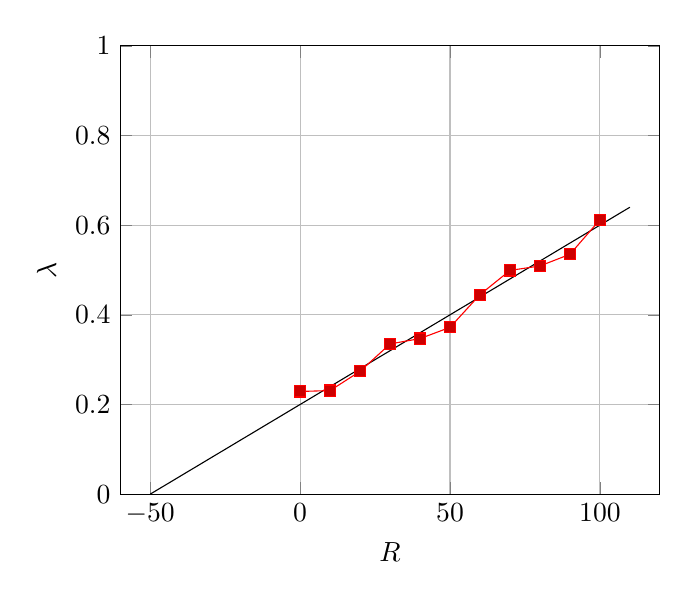
\begin{tikzpicture}
	\begin{axis}[
	xlabel=$R$,
	ylabel=$\lambda$,
	xmin=-60, xmax= 120,
	ymin=0, ymax=1,
	grid=major
	]
	\addplot[domain=-50:110, samples=100] {0.004*x + 0.2};
	\addplot coordinates {
		(0, 0.229)
		(10, 0.231)
		(20, 0.274)
		(30, 0.335)
		(40, 0.347)
		(50, 0.372)
		(60, 0.445)
		(70, 0.499)
		(80, 0.509)
		(90, 0.535)
		(100, 0.612)
	};
	\end{axis}
	\end{tikzpicture}
\end{figure}

\begin{figure}[h]
	\centering
	\caption{График зависимости Q от R}
	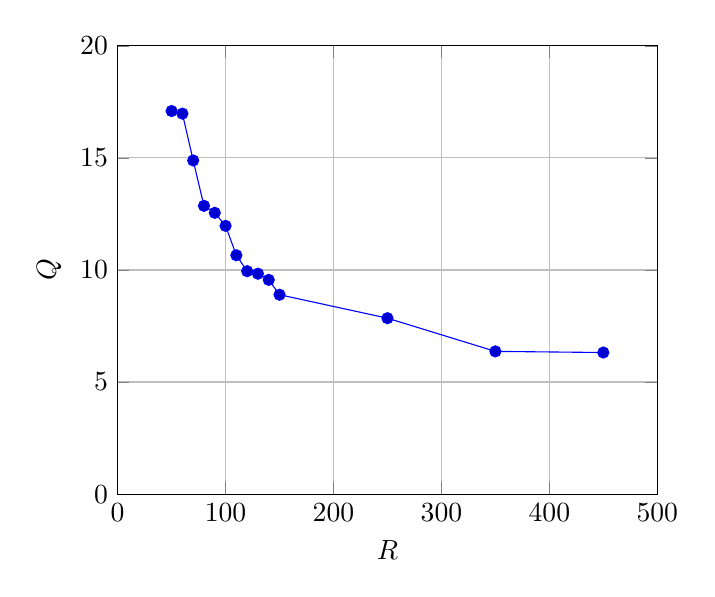
\begin{tikzpicture}
	\begin{axis}[
	xlabel=$R$,
	ylabel=$Q$,
	xmin=0, xmax=500,
	ymin=0, ymax=20,
	grid=major
	]
	\addplot coordinates {
		(50, 17.09064326)
		(60, 16.97399783)
		(70, 14.88521548)
		(80, 12.86117207)
		(90, 12.54930227)
		(100, 11.96667483)
		(110, 10.65591126)
		(120, 9.946402453)
		(130, 9.83273164)
		(140, 9.558723616)
		(150, 8.895834376)
		(250, 7.848897368)
		(350, 6.368152179)
		(450, 6.317377144)
	};
	\end{axis}
	\end{tikzpicture}
\end{figure}